
%% bare_conf.tex
%% V1.4b
%% 2015/08/26
%% by Michael Shell
%% See:
%% http://www.michaelshell.org/
%% for current contact information.
%%
%% This is a skeleton file demonstrating the use of IEEEtran.cls
%% (requires IEEEtran.cls version 1.8b or later) with an IEEE
%% conference paper.
%%
%% Support sites:
%% http://www.michaelshell.org/tex/ieeetran/
%% http://www.ctan.org/pkg/ieeetran
%% and
%% http://www.ieee.org/

%%*************************************************************************
%% Legal Notice:
%% This code is offered as-is without any warranty either expressed or
%% implied; without even the implied warranty of MERCHANTABILITY or
%% FITNESS FOR A PARTICULAR PURPOSE! 
%% User assumes all risk.
%% In no event shall the IEEE or any contributor to this code be liable for
%% any damages or losses, including, but not limited to, incidental,
%% consequential, or any other damages, resulting from the use or misuse
%% of any information contained here.
%%
%% All comments are the opinions of their respective authors and are not
%% necessarily endorsed by the IEEE.
%%
%% This work is distributed under the LaTeX Project Public License (LPPL)
%% ( http://www.latex-project.org/ ) version 1.3, and may be freely used,
%% distributed and modified. A copy of the LPPL, version 1.3, is included
%% in the base LaTeX documentation of all distributions of LaTeX released
%% 2003/12/01 or later.
%% Retain all contribution notices and credits.
%% ** Modified files should be clearly indicated as such, including  **
%% ** renaming them and changing author support contact information. **
%%*************************************************************************


% *** Authors should verify (and, if needed, correct) their LaTeX system  ***
% *** with the testflow diagnostic prior to trusting their LaTeX platform ***
% *** with production work. The IEEE's font choices and paper sizes can   ***
% *** trigger bugs that do not appear when using other class files.       ***                          ***
% The testflow support page is at:
% http://www.michaelshell.org/tex/testflow/



\documentclass[conference]{IEEEtran}
% Some Computer Society conferences also require the compsoc mode option,
% but others use the standard conference format.
%
% If IEEEtran.cls has not been installed into the LaTeX system files,
% manually specify the path to it like:
% \documentclass[conference]{../sty/IEEEtran}





% Some very useful LaTeX packages include:
% (uncomment the ones you want to load)


% *** MISC UTILITY PACKAGES ***
%
%\usepackage{ifpdf}
% Heiko Oberdiek's ifpdf.sty is very useful if you need conditional
% compilation based on whether the output is pdf or dvi.
% usage:
% \ifpdf
%   % pdf code
% \else
%   % dvi code
% \fi
% The latest version of ifpdf.sty can be obtained from:
% http://www.ctan.org/pkg/ifpdf
% Also, note that IEEEtran.cls V1.7 and later provides a builtin
% \ifCLASSINFOpdf conditional that works the same way.
% When switching from latex to pdflatex and vice-versa, the compiler may
% have to be run twice to clear warning/error messages.






% *** CITATION PACKAGES ***
%
%\usepackage{cite}
% cite.sty was written by Donald Arseneau
% V1.6 and later of IEEEtran pre-defines the format of the cite.sty package
% \cite{} output to follow that of the IEEE. Loading the cite package will
% result in citation numbers being automatically sorted and properly
% "compressed/ranged". e.g., [1], [9], [2], [7], [5], [6] without using
% cite.sty will become [1], [2], [5]--[7], [9] using cite.sty. cite.sty's
% \cite will automatically add leading space, if needed. Use cite.sty's
% noadjust option (cite.sty V3.8 and later) if you want to turn this off
% such as if a citation ever needs to be enclosed in parenthesis.
% cite.sty is already installed on most LaTeX systems. Be sure and use
% version 5.0 (2009-03-20) and later if using hyperref.sty.
% The latest version can be obtained at:
% http://www.ctan.org/pkg/cite
% The documentation is contained in the cite.sty file itself.






% *** GRAPHICS RELATED PACKAGES ***
%
\ifCLASSINFOpdf
  % \usepackage[pdftex]{graphicx}
  % declare the path(s) where your graphic files are
  % \graphicspath{{../pdf/}{../jpeg/}}
  % and their extensions so you won't have to specify these with
  % every instance of \includegraphics
  % \DeclareGraphicsExtensions{.pdf,.jpeg,.png}
\else
  % or other class option (dvipsone, dvipdf, if not using dvips). graphicx
  % will default to the driver specified in the system graphics.cfg if no
  % driver is specified.
  % \usepackage[dvips]{graphicx}
  % declare the path(s) where your graphic files are
  % \graphicspath{{../eps/}}
  % and their extensions so you won't have to specify these with
  % every instance of \includegraphics
  % \DeclareGraphicsExtensions{.eps}
\fi
% graphicx was written by David Carlisle and Sebastian Rahtz. It is
% required if you want graphics, photos, etc. graphicx.sty is already
% installed on most LaTeX systems. The latest version and documentation
% can be obtained at: 
% http://www.ctan.org/pkg/graphicx
% Another good source of documentation is "Using Imported Graphics in
% LaTeX2e" by Keith Reckdahl which can be found at:
% http://www.ctan.org/pkg/epslatex
%
% latex, and pdflatex in dvi mode, support graphics in encapsulated
% postscript (.eps) format. pdflatex in pdf mode supports graphics
% in .pdf, .jpeg, .png and .mps (metapost) formats. Users should ensure
% that all non-photo figures use a vector format (.eps, .pdf, .mps) and
% not a bitmapped formats (.jpeg, .png). The IEEE frowns on bitmapped formats
% which can result in "jaggedy"/blurry rendering of lines and letters as
% well as large increases in file sizes.
%
% You can find documentation about the pdfTeX application at:
% http://www.tug.org/applications/pdftex





% *** MATH PACKAGES ***
%
%\usepackage{amsmath}
% A popular package from the American Mathematical Society that provides
% many useful and powerful commands for dealing with mathematics.
%
% Note that the amsmath package sets \interdisplaylinepenalty to 10000
% thus preventing page breaks from occurring within multiline equations. Use:
%\interdisplaylinepenalty=2500
% after loading amsmath to restore such page breaks as IEEEtran.cls normally
% does. amsmath.sty is already installed on most LaTeX systems. The latest
% version and documentation can be obtained at:
% http://www.ctan.org/pkg/amsmath





% *** SPECIALIZED LIST PACKAGES ***
%
%\usepackage{algorithmic}
% algorithmic.sty was written by Peter Williams and Rogerio Brito.
% This package provides an algorithmic environment fo describing algorithms.
% You can use the algorithmic environment in-text or within a figure
% environment to provide for a floating algorithm. Do NOT use the algorithm
% floating environment provided by algorithm.sty (by the same authors) or
% algorithm2e.sty (by Christophe Fiorio) as the IEEE does not use dedicated
% algorithm float types and packages that provide these will not provide
% correct IEEE style captions. The latest version and documentation of
% algorithmic.sty can be obtained at:
% http://www.ctan.org/pkg/algorithms
% Also of interest may be the (relatively newer and more customizable)
% algorithmicx.sty package by Szasz Janos:
% http://www.ctan.org/pkg/algorithmicx




% *** ALIGNMENT PACKAGES ***
%
%\usepackage{array}
% Frank Mittelbach's and David Carlisle's array.sty patches and improves
% the standard LaTeX2e array and tabular environments to provide better
% appearance and additional user controls. As the default LaTeX2e table
% generation code is lacking to the point of almost being broken with
% respect to the quality of the end results, all users are strongly
% advised to use an enhanced (at the very least that provided by array.sty)
% set of table tools. array.sty is already installed on most systems. The
% latest version and documentation can be obtained at:
% http://www.ctan.org/pkg/array


% IEEEtran contains the IEEEeqnarray family of commands that can be used to
% generate multiline equations as well as matrices, tables, etc., of high
% quality.




% *** SUBFIGURE PACKAGES ***
%\ifCLASSOPTIONcompsoc
%  \usepackage[caption=false,font=normalsize,labelfont=sf,textfont=sf]{subfig}
%\else
%  \usepackage[caption=false,font=footnotesize]{subfig}
%\fi
% subfig.sty, written by Steven Douglas Cochran, is the modern replacement
% for subfigure.sty, the latter of which is no longer maintained and is
% incompatible with some LaTeX packages including fixltx2e. However,
% subfig.sty requires and automatically loads Axel Sommerfeldt's caption.sty
% which will override IEEEtran.cls' handling of captions and this will result
% in non-IEEE style figure/table captions. To prevent this problem, be sure
% and invoke subfig.sty's "caption=false" package option (available since
% subfig.sty version 1.3, 2005/06/28) as this is will preserve IEEEtran.cls
% handling of captions.
% Note that the Computer Society format requires a larger sans serif font
% than the serif footnote size font used in traditional IEEE formatting
% and thus the need to invoke different subfig.sty package options depending
% on whether compsoc mode has been enabled.
%
% The latest version and documentation of subfig.sty can be obtained at:
% http://www.ctan.org/pkg/subfig




% *** FLOAT PACKAGES ***
%
%\usepackage{fixltx2e}
% fixltx2e, the successor to the earlier fix2col.sty, was written by
% Frank Mittelbach and David Carlisle. This package corrects a few problems
% in the LaTeX2e kernel, the most notable of which is that in current
% LaTeX2e releases, the ordering of single and double column floats is not
% guaranteed to be preserved. Thus, an unpatched LaTeX2e can allow a
% single column figure to be placed prior to an earlier double column
% figure.
% Be aware that LaTeX2e kernels dated 2015 and later have fixltx2e.sty's
% corrections already built into the system in which case a warning will
% be issued if an attempt is made to load fixltx2e.sty as it is no longer
% needed.
% The latest version and documentation can be found at:
% http://www.ctan.org/pkg/fixltx2e


%\usepackage{stfloats}
% stfloats.sty was written by Sigitas Tolusis. This package gives LaTeX2e
% the ability to do double column floats at the bottom of the page as well
% as the top. (e.g., "\begin{figure*}[!b]" is not normally possible in
% LaTeX2e). It also provides a command:
%\fnbelowfloat
% to enable the placement of footnotes below bottom floats (the standard
% LaTeX2e kernel puts them above bottom floats). This is an invasive package
% which rewrites many portions of the LaTeX2e float routines. It may not work
% with other packages that modify the LaTeX2e float routines. The latest
% version and documentation can be obtained at:
% http://www.ctan.org/pkg/stfloats
% Do not use the stfloats baselinefloat ability as the IEEE does not allow
% \baselineskip to stretch. Authors submitting work to the IEEE should note
% that the IEEE rarely uses double column equations and that authors should try
% to avoid such use. Do not be tempted to use the cuted.sty or midfloat.sty
% packages (also by Sigitas Tolusis) as the IEEE does not format its papers in
% such ways.
% Do not attempt to use stfloats with fixltx2e as they are incompatible.
% Instead, use Morten Hogholm'a dblfloatfix which combines the features
% of both fixltx2e and stfloats:
%
% \usepackage{dblfloatfix}
% The latest version can be found at:
% http://www.ctan.org/pkg/dblfloatfix




% *** PDF, URL AND HYPERLINK PACKAGES ***
%
%\usepackage{url}
% url.sty was written by Donald Arseneau. It provides better support for
% handling and breaking URLs. url.sty is already installed on most LaTeX
% systems. The latest version and documentation can be obtained at:
% http://www.ctan.org/pkg/url
% Basically, \url{my_url_here}.




% *** Do not adjust lengths that control margins, column widths, etc. ***
% *** Do not use packages that alter fonts (such as pslatex).         ***
% There should be no need to do such things with IEEEtran.cls V1.6 and later.
% (Unless specifically asked to do so by the journal or conference you plan
% to submit to, of course. )



\usepackage[onelanguage,linesnumbered,ruled,inoutnumbered]{algorithm2e}


\usepackage{graphicx}


% correct bad hyphenation here
\hyphenation{op-tical net-works semi-conduc-tor}


\usepackage{syntax}
\grammarindent 80pt

\usepackage{newfloat}
% declare the floating environment {Grammar}
% this will also define \listofGrammars:
\DeclareFloatingEnvironment[
% the file extension for the file used to create the list:
fileext   = logr,% don't use log here!
% the heading for the list:
listname  = {List of Grammars},
% the name used in captions:
name      = Grammar,
% the default floating parameters if the environment is used
% without optional argument:
placement = htp
]{Grammar}




\begin{document}
%
% paper title
% Titles are generally capitalized except for words such as a, an, and, as,
% at, but, by, for, in, nor, of, on, or, the, to and up, which are usually
% not capitalized unless they are the first or last word of the title.
% Linebreaks \\ can be used within to get better formatting as desired.
% Do not put math or special symbols in the title.
\title{Automated Design of Hyper-Heuristics Components Applied to the PSP Problem}


% author names and affiliations
% use a multiple column layout for up to three different
% affiliations

\author{\IEEEauthorblockN{Vidal D. Fontoura}
\IEEEauthorblockA{Federal University of Parana \\ (DInf-UFPR), Curitiba - PR, Brazil\\
Email: vdfontoura@inf.ufpr.br}
\and
\IEEEauthorblockN{Aurora T. R. Pozo}
\IEEEauthorblockA{Federal University of Parana \\ (DInf-UFPR), Curitiba - PR, Brazil\\
Email: aurora@inf.ufpr.br}
\and
\IEEEauthorblockN{Roberto Santana Hermida}
\IEEEauthorblockA{University of the Basque Country\\
Barrio Sarriena s/n 48940 Leioa Bizkaia\\
Email: roberto.santana@ehu.es
}}

% conference papers do not typically use \thanks and this command
% is locked out in conference mode. If really needed, such as for
% the acknowledgment of grants, issue a \IEEEoverridecommandlockouts
% after \documentclass

% for over three affiliations, or if they all won't fit within the width
% of the page, use this alternative format:
% 
%\author{\IEEEauthorblockN{Michael Shell\IEEEauthorrefmark{1},
%Homer Simpson\IEEEauthorrefmark{2},
%James Kirk\IEEEauthorrefmark{3}, 
%Montgomery Scott\IEEEauthorrefmark{3} and
%Eldon Tyrell\IEEEauthorrefmark{4}}
%\IEEEauthorblockA{\IEEEauthorrefmark{1}School of Electrical and Computer Engineering\\
%Georgia Institute of Technology,
%Atlanta, Georgia 30332--0250\\ Email: see http://www.michaelshell.org/contact.html}
%\IEEEauthorblockA{\IEEEauthorrefmark{2}Twentieth Century Fox, Springfield, USA\\
%Email: homer@thesimpsons.com}
%\IEEEauthorblockA{\IEEEauthorrefmark{3}Starfleet Academy, San Francisco, California 96678-2391\\
%Telephone: (800) 555--1212, Fax: (888) 555--1212}
%\IEEEauthorblockA{\IEEEauthorrefmark{4}Tyrell Inc., 123 Replicant Street, Los Angeles, California 90210--4321}}




% use for special paper notices
%\IEEEspecialpapernotice{(Invited Paper)}




% make the title area
\maketitle

% As a general rule, do not put math, special symbols or citations
% in the abstract
\begin{abstract}
Proteins are structures, composed by amino-acids, and have an important role in nature. These structures are formed by a process called protein folding. This process is not completely understood and it is considered one of the most challenging modern problems. This problem is usually called as Protein Structure Prediction (PSP) and can be considered as a minimization problem. Hence, many heuristics strategies have been applied in order to find protein structures that minimizes its free energy. However, these strategies have difficulties on finding the optimal solutions to the longer sequences of amino-acids, due, the complexity of the problem and the huge amount of local optima. The hyper-heuristics framework are usually useful in this kind of context since they try to combine different heuristics strengths into a single framework. Moreover, there is lack of works whose aim the automated design of hyper-heuristics components. Sabar et al. \cite{sabar2015automatic} proposed the automated design of high level heuristics to a hyper-heuristic framework and evaluated its performance by applying in the 6 domain problems from HyFlex \cite{ochoa2012hyflex} framework. The work of Sabar et al. \cite{sabar2015automatic} influenced this paper to chase the generation of high level components to a hyper-heuristic framework to the PSP problem.
\end{abstract}

% no keywords




% For peer review papers, you can put extra information on the cover
% page as needed:
% \ifCLASSOPTIONpeerreview
% \begin{center} \bfseries EDICS Category: 3-BBND \end{center}
% \fi
%
% For peerreview papers, this IEEEtran command inserts a page break and
% creates the second title. It will be ignored for other modes.
\IEEEpeerreviewmaketitle



\section{Introduction}
Proteins plays a fundamental role in nature, they are involved in many important functions for  the living cells. Proteins are structures, composed by amino-acids that guarantees the correct operation of wide range of biological entities. These structures are result from a process so-called protein folding, in which initially an unfolded chain of amino-acids will be transformed into its final/native structure.

The protein structure prediction (PSP) has a wide range of biotechnology and medical applications. For instance: synthesis of new proteins and folds \cite{wang2012structural, rothlisberger2008kemp}, structure based synthesis of new drugs \cite{davis2009rosettaligand}, refinement of theoretical models obtained by comparative modeling \cite{qian2004improvement, krieger2009improving}, and
obtaining experimental structures from incomplete nuclear magnetic
resonance data  \cite{shen2009novo}.  

The determination of the native structure of a protein is a hard task even for the modern super computers. The difficulty is due to the huge search space to test all possible configurations that a given protein can adopt. Many models to represent the proteins structures exists and can be utilized to simulated the folding process. Although there exists extremely detailed models, these representations are computational very expensive. Hence, many authors \cite{custodio2004investigation,hsu2003growth,lin2011protein,unger1993genetic,santana2008protein,custodio2014multiple, garza2012locality} used simplified models to represent the protein structures. A useful model for this purpose is the Hydrophobic-Polar (HP) model presented by Lau and Dill \cite{lau1989lattice}. This model generalizes the amino-acids that composes the proteins into just two types H or P. And, a grid (2D) or cube (3D) can be used to represent the conformations that a protein can adopt. Each conformation has an energy associated \cite{unger1993genetic}. 

% Para isto, é necessário considerar as interações entre os aminoácidos. Uma interação ocorre quando o par de aminoácidos é adjacente no \textit{grid}/cubo e não é adjacente na sequência. No modelo HP existem apenas três: (HP, HH e PP), mas somente interações hidrofóbicas (HH) influenciam no valor de energia referente a uma conformação \cite{unger1993genetic}. A questão que surge é como buscar, dentre as possíveis conformações, aquela cuja a energia seja mínima.

Many heuristics strategies were developed to find conformations of minimum energy, using the HP model. These approaches use genetic algorithms \cite{unger1993genetic}, ant colony optimization \cite{shmygelska2002ant, shmygelska2003improved}, estimation distribution algorithms \cite{santana2008protein }, among others\cite{gabriel2012algoritmos}

 Although, there are different strategies already proposed for the PSP, all of them face difficulties to reach the optimal configurations when the length of amino-acids sequences increases. This motivate the study here presented. The goal is to use a pool of heuristics proposed in the literature managed by a hyper-heuristic strategy \cite{burke2013hyper}.  Hence, different heuristics have different strengths and weakness. It makes sense to merge them into one framework and let a high-level strategy to manage the application of them. 

 Burke et al. \cite{burke2010classification} recently defined hyper-heuristics as "an automated methodology for selecting or generating heuristics to solve hard computational search problems". Over the years, these methodologies have demonstrated success in solving a wide range of real world problems.  However, there are a lack of works that use this approach to solve the PSP problem.

The paper describes the automated generation of hyper-heuristics to solve the PSP problem. The hyper-heuristic includes two main components:  a selection mechanisms and acceptance criteria.  Both components are generated using grammatical evolution (GE), which is a kind of genetic programming (GP). A set of experiment was designed to evaluate the approach using eleven PSP instances. The results are compared with the previous works of the literature.  



This paper is organized as follows: in the next section we briefly introduce the Protein Structure Prediction problem and a review of the related works is also presented.  Section \ref{sec:background} presents a background of hyper-heuristics, genetic programming and the grammatical evolution algorithm. Thereafter, in Section \ref{sec:methodology} the proposed methodology of this paper is presented. In Section \ref{sec:experiments}, the experimental benchmark and numerical results of the conducted experiments are presented. Finally, in Section \ref{sec:conclusion}, the conclusions of the research are given, and further work is discussed.


%TODO: if this is necessary
%The propose of this paper is based on a previous work developed by Sabar et al. \cite{sabar2015automatic}, which generates high level heuristics to six domain problems contained in the hyper-heuristic framework HyFlex \cite{ochoa2012hyflex}.

\section{Protein Structure Prediction} \label{sec:proteinfolding}


Proteins are macromolecules composed by an alphabet of twenty different amino acids, also referred to as residues. An amino acid is formed by a peptide backbone and a distinctive side chain group. The peptide bond is defined by an amino group and a carboxyl group connected to an alpha carbon to which a hydrogen and side chain group are attached.


Sequences are formed by combining amino acids and are considered the primary structure of
proteins.
%Amino acids are combined to form sequences which are considered the primary structure of the peptides or proteins. 
The secondary structure is the locally ordered structure brought via hydrogen bounding mainly within the peptide backbone. The most common secondary structure elements in proteins are the alpha helix and the beta sheet. The global folding of a polypeptide chain is also called as the tertiary structure.

%The tertiary structure is the global folding of a single polypeptide chain.

Under specific conditions, the protein sequence folds into a unique native 3-D structure. Each possible protein fold has an associated energy value. The \emph{thermodynamic hypothesis} states that the native structure of a protein is the one for which the free energy achieves the global minimum. Based on this hypothesis, many methods \cite{custodio2004investigation, hsu2003growth, krasnogor2002multimeme, lin2011protein, unger1993genetic} that search for the protein native structure define an approximation of the protein energy and use optimization algorithms that look for the protein fold that minimizes the energy. These approaches mainly differ in the type of energy approximation employed and in the characteristics of the protein modeling.


\subsection{The HP Model} \label{sec:hpModel}


%Using a representation close to the real would be impossible for current computers to process the information in a reasonable time.
The protein structures are very complex. Detailed representations of proteins exists and can be used to model the protein folding, these representations are computationally very costly. Having this in mind, Lau and Dill \cite{lau1989lattice} created a model called \textit{Hydrophobic-Hydrophilic} Model (HP Model), to represent the proteins using simplifications. The model can be used either to represent proteins in a 2D space or 3D space.


The HP model considers two types of residues:  hydrophobic (H) residues  and hydrophilic or polar (P) residues. A protein is considered a sequence of these two types of residues, which are located in regular lattice models forming self-avoided paths. Given a pair of residues, they are considered neighbors if they are adjacent  either in the chain (connected neighbors) or  in the lattice but not connected in the chain (topological neighbors).


\begin{figure}[htb!] \label{fig:PROTEXAM}
	\centering
	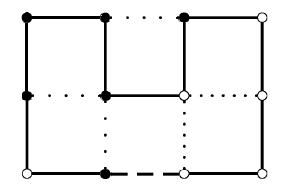
\includegraphics[scale=0.7]{figures/proteinExample.png}
	\caption{One possible configuration of  sequence $PPPPHPHHHHPH$ in the HP model. There is one $HH$ (represented by a dotted line with wide spaces), one $HP$ (represented by a dashed line) and  two $PP$  (represented by dotted lines) contacts.}
\end{figure}


%The total number of topological neighboring positions in the lattice ($z$) is called the lattice coordination number.


For the HP model, an energy function that  measures the interaction between topological  neighbor residues is defined  as  $\epsilon_{HH}=-1$ and $\epsilon_{HP}=\epsilon_{PP}=0$. The HP problem consists of finding the solution that minimizes the total energy. In the linear representation of the sequence, hydrophobic residues are represented with the letter H and polar ones, with P. In the graphical representation, hydrophobic proteins are represented  by black beads and polar proteins, by white beads.  Figure 1 shows the graphical representation of a possible configuration for  the sequence  $PPPPHPHHHHPH$ in a 2D space. The energy that the HP model associates with this configuration is $-2$ TODO: fixme because there is only two $HH$ contact, arisen between the second and fifth residues.


Among many works that explores the PSP problem, here are some examples of the approaches that have been used to solve it.

A very influential paper from Unger and Moult  \cite{unger1993genetic}, introduces a evolutionary algorithm (EA) which uses heuristic-based crossover and mutation operators for the HP model. The algorithm outperformed many variants of Monte Carlo methods for different instances. However,
good results were obtained, the EA was unable to find the global optimal for the longest instances considered.

%
%Alternative
%Unger and Moult \cite{unger1993genetic} described a genetic algorithm (GA) that uses heuristic-based operators for crossover and mutation for the HP model.



A multimeme algorithm (MMA) presented in \cite{krasnogor2002multimeme} is a EA combined with a
group of local search methods. For each individual in the population the MMA, selects a local search method that best fits. Used first to find solutions for the functional model protein. The strategy was later improved with fuzzy-logic-based local searches, leading the algorithm to achieve improved results in the PSP problem.

%The multimeme algorithm (MMA) proposed by \cite{krasnogor2002multimeme} is a GA combined with a set of local search methods. The algorithm, for each different instance or individual in the population, selects the local search method that best fits. 




%Originally used to find solutions for the functional model protein. The algorithm was later improved with fuzzy-logic-based local searches, leading the algorithm to produce improved results in the PSP problem.


In \cite{hsu2003growth}, the author uses  pruned-enriched Rosenbluth method (PERM) also know as Chain growth algorithm, that is based on growing the sequence conformation by adding particle by particle, aiming to increase good configurations and eliminating bad ones.


The ant colony optimization (ACO) was applied to the PSP problem using the HP-2D model in \cite{shmygelska2002ant, shmygelska2003improved}. This strategy, uses artificial ants to build conformations for a given HP instance. A local search method is then applied to further improve the solutions and also maintain the quality of the solutions.

The work of \cite{santana2008protein} utilizes Estimation of distribution algorithms (EDAs) as an efficient evolutionary algorithm that learns and exploits the search space in the form of probabilistic dependencies. New ideas were introduced 
for the application of EDAs to 2D and 3D simplified protein folding problem. The relationship between this proposal and other population-based approaches for the PSP was analyzed. The obtained results showed that EDAs can achieve superior solutions compared with other well-known population based optimization algorithms.



%TODO: Multi Objective, maybe replace with another work, probably the Sabar one should be a good option here
%Gabriel \textit{et al}. \cite{gabriel2012algoritmos} propose the use of a table-based multi objective evolutionary algorithm initially introduced by \cite{delbem2002restabelecimento}, using the HP-3D model for the representation and solution evaluation. The authors also propose the use of a second objective that aims to measure the distance between hydrophobic amino-acids, allowing the algorithm to distinguish between different solutions with the same energy value.

%TODO: check how to improve it
The present paper proposes the use of a grammatical evolution GE to generate high level heuristics for a hyper heuristic framework that will be applied to the PSP problem.
\section{Background}
\label{sec:background}

This section will present the background context in order to supply the readers with the necessary information, for a good comprehension of the concepts and techniques used by this paper.  


\subsection{Hyper-Heuristics}

%Hyper-Heuristics can be seen as a methodology to select or create heuristics for a given moment of the search. 

 Burke et al. \cite{burke2010classification} recently defined hyper-heuristics as "an automated methodology for selecting or generating heuristics to solve hard computational search problems". Mainly, a generic hyper-heuristic framework is composed of two main components known as high-level and low-level heuristics. Figure \ref{fig:HyperHeuristics} shows a general scheme of hyper-heuristic frameworks. The high and low level are separated by a domain barrier which means that the low-level component is problem dependent while the high-level component does not require any knowledge of the problem domain. Ideally, to apply a hyper-heuristic framework to a different problem domain: it is possible to do it only by replacing  the low-level component no changes should be required at the high-level. It is responsibility from the high-level component to manage the selection or generation of which heuristic should be applied at each decision point. The low-level component corresponds to a pool of heuristics or heuristic components \cite{sabar2015automatic}. 
 
 
\begin{figure}[htb!] \label{fig:HyperHeuristics}
	\centering
	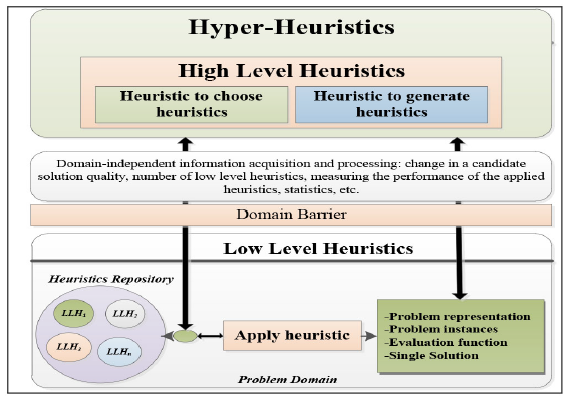
\includegraphics[scale=0.6]{figures/hyperheuristic.png}
	\caption{General scheme of hyper-heuristic framework}
\end{figure}	



%Recently Burke et al. \cite{burke2010classification} classified hyper-heuristic frameworks based on the source of feedback during the learning process and the nature of the search space. In the case of the source of feedback Burke el al. \cite{burke2010classification} mention 3 possibilities: online, offline and no learning. If the hyper-heuristic framework uses information gathered during the problem solving it is considered as an online framework. An offline framework requires a training phase to gather information in order to use later in the validation phase. No learning occurs when no feedback is provided to the hyper-heuristic framework \cite{sabar2015automatic}. The nature of the search space can be either selecting or generating heuristics for the underlying problem. Next will be analyzed both kinds of high-level heuristics.

Recently Burke et al. \cite{burke2010classification} classified the hyper-heuristics framework based on the nature of the search space: can be either selecting or generating heuristics for the underlying problem. Next will be analyzed both kinds of high-level heuristics.


\begin{itemize}
	\item Selecting Heuristics: The majority of hyper-heuristic frameworks published define high level heuristics to select low level heuristics. In general, these frameworks define a selection mechanism and also a acceptance criterion. These strategies uses information from the historical of low level heuristics applications. For instance a greedy selection considers only the number of improvements that a low level heuristic obtained. In contrast, the choice function \cite{burke2013hyper} is a reward-based strategy, which considers both the number of improvements and the elapsed time since the last application.
	
	
%	Using statistical information (e.g: number of improvements, rewards , number of accepts, amount of improvement) related with the low level heuristics applications, the high level heuristics are made of.
	%TODO: maybe change to built out
	
	
	
	
	
	
	
%	The pool can contain both constructive or perturbative heuristics. 
%	
	
%	The objective of the hyper-heuristic framework is to select the heuristic, from the pool, which most suits at a given moment. The main idea behind this: the strength of several heuristics can be combined into a single framework in order to better explore the search space. 
%	Most of the proposed selection mechanisms use simple rules to select the low level heuristics based on their past performance \cite{sabar2015automatic}.

	\item Generating Heuristics: In this case, the hyper-heuristic framework starts with a set subcomponents from low level heuristics and have the goal of fabricate new low level heuristics with it. Genetic programming is reported as a good strategy to combine and generated new heuristics for the SAT, scheduling and bin-packing problems \cite{sabar2015automatic}.
\end{itemize}

A novel work presented by Sabar et al. \cite{sabar2015automatic}, uses GEP (gene expression programming a kind of genetic programming) with the goal of generating the components (high level heuristics) to a hyper-heuristic framework. The experiments presented by Sabar et al. \cite{sabar2015automatic}, using the 6 problem domains provided by the HyFlex hyper-heuristic framework, shown a impressive results comparing with other human-designed hyper-heuristic strategies from the state of art. This work inspired the present paper which has the objective of generating selection mechanism and acceptance criteria, through a grammatical evolution process, to a hyper-heuristic framework. 



\subsection{Genetic Programming {GP}}
 Is a sub-field from the program synthesis which uses ideas from the evolution theory to produce programs \cite{burke2013hyper}. 

% The main factors from the evolutionary computation are inheritance, reproduction/mutation and selection of the fittest. Initially, a random-generated population of programs is created. Using a selection method to select good individuals for reproduction. Then the reproduction and mutation steps takes place in order to generate an offspring. Finally, the offspring is evaluated to assign a fitness value and based on this value the offspring can either enter or not in the population. 

%Traditionally, in genetic programming, the programs that compose the population are represented using a tree structure. However, other structures that can be evolved exists, for instance: linear sequences of instructions and grammar expressions. 

\subsubsection{Grammatical Evolution (GE)} 

Is a relatively new technique from the evolutionary computing, introduced by Ryan el al. \cite{ryan1998grammatical} and it is a type of GP which utilizes a grammar to generate programs. Just like in GP the main goal is to find a executable program or piece of code, which have a good fitness value. Ryan el al. \cite{ryan1998grammatical} proposes a technique to generate programs or fragments for any language using BNF (Backus Naur Form) definitions. This technique can be used to evolve programs though a evolution process. The GE uses a mapping mechanism between the genotype (coded individuals by integer vectors) and phenotype (generated programs to resolve a problem). The BNF notation is used to represent a grammar from a language in form of production rules. A BNF grammar consists in a set of terminals, which are items that are allowed to the language, for instance: +, -, *, / etc and non-terminals, which can be expanded into one or more terminals. The grammar can be expressed as a tuple ${N,T,P,S}$, where $N$ is a set of non-terminals, $T$ a set of terminals, $P$ a set of production rules that maps the elements $N$ to $T$; finally, $S$, a symbol to represent the initial point contained in $N$.
 
\begin{center}
	
	$ N = {\langle expr \rangle, \langle op \rangle, \langle pre-op \rangle}$
	
	$ T = {Sin,Cos,Tan,Log,+,-,/,*,X} $
	
	$ S = \langle expr \rangle $
	
\end{center}

\noindent
And $P$ can be represented as:

\begin{Grammar}
	\begin{grammar}
		
		
		<expr> ::=  <expr> <op> <expr> \hspace{2cm} (0) 
		\alt (<expr> <op> <expr>)  \hspace{1.75cm}  (1)  
		\alt <pre-op> (<expr>) \hspace{2.2cm}  (2) \alt <var> \hspace{3.9cm} (3) \\\
		
		<op> ::=  + \hspace{4.4cm} (0)   \alt - \hspace{4.5cm}  (1)  \alt  /  \hspace{4.51cm}  (2) \alt * \hspace{4.45cm}  (3) \\
		
		<pre-op> ::= Sin \hspace{4.2cm} (0) \alt Cos
	\hspace{4.12cm} (1) \alt Tan  \hspace{4.13cm} (2) \alt Cos \hspace{4.12cm} (3) \\
		
		<var> ::= X  \hspace{4.4cm} (0)
		
		
	\end{grammar}
	
	\caption{Sample grammar to demonstrate how to decode integer vectors in computer programs}
	\label{gram:gramatica}
\end{Grammar}


\begin{table}[htb]
	\centering
	\caption{Production rules and the number of choices allowed}
	\label{tab:productionRules}
	\begin{tabular}{|l|l|}
		\hline
		Production Rules & Number of choices \\ \hline
		$\langle expr \rangle$                        & 4       \\ \hline
		$\langle op \rangle$                         & 4       \\ \hline
		$\langle pre-op \rangle$                         & 4       \\ \hline
		$\langle var \rangle$                          & 1       \\ \hline
	\end{tabular}
\end{table}


Ryan et al. \cite{ryan1998grammatical}  proposed the use of genetic algorithm (GA) to control which choices should be made, in this sense allowing the GA to select which production rules should be utilized. An individual (chromosome) consists in variable-length integer vector and it is called genotype. Algorithm \ref{alg:GE} presents the pseudo code of a grammatical evolution program. Except for lines 11, 12 and the introduction of grammar file to decode the integer vectors into programs, the GE looks very similar to a simple GA.

\begin{algorithm}[htb]
	\fontsize{8pt}{10pt}\selectfont
	\caption{Pseudo code from the Grammatical Evolution}
	\label{alg:GE}
	\KwIn{GF -- Grammar File}
	\Begin{
		$population \gets$ Create population\;
		$programas \gets$ Maps the $population$ to programs using $GF$\;
		Execute the $program$\;
		Assign fitness value to the solutions of $population$ according with the output obtained by the respective decoded program\;
		\While{Stop condition not reached}{
			$parents \gets $ Select individuals to crossover\;
			$offspring \gets$ Crossover($pais$)\;		
			$populacao \gets$  Replacement\;
			
			Apply the \textit{Prune} operator to the $offspring$\;
			Apply the \textit{Duplicate} operator  to the $offspring$\;
			Apply the \textit{Mutation} operator to the $offspring$\;
			$programs \gets$ Maps $offspring$ to programs using $GF$\;
			Execute $programs$\;
			Assign \textit{fitness} value to solutions $offspring$ according with the output obtained by the respective decoded program\;
			$population \gets$ Replacement\;
		}
		\Return{Best program from the $population$}\;
	}
\end{algorithm}


For the sake of comprehension the chromosome mapping process will be demonstrated using the Grammar \ref{gram:gramatica}. The Algorithm \ref{alg:pseudocodigogrammar} presents the general template of the generated programs. The expression $\langle expr \rangle$ presented in line 2 is replaced by mathematical expressions coded by the chromosomes (integer vectors).


\begin{algorithm}
	\caption{General template for the generated algorithms}
	\label{alg:pseudocodigogrammar}
	float symb(float x) { \\
		a = $\langle expr \rangle$;   \\
		return a;  \\
	}	
\end{algorithm}


\noindent
Now suppose the following integer vector:

\begin{center}
	$ [220, 203, 17, 6, 108, 215, 104, 30] $
\end{center}

This vector will be utilized to decode the chromosome (genotype) into a piece of code (phenotype)  using the BNF grammar.
Table \ref{tab:productionRules} summarizes the number of choices associated within each production rule from Grammar \ref{gram:gramatica}. There are 4 options of production rules that can be selected for the expression $ \langle expr \rangle$. In order to select which option, the first value from the vector should be used. The value is 220 and its mod divided by 4 (four options that can be selected for the expression $ \langle expr \rangle$) results in 0, which means that the first option should be selected $\langle expr \rangle \langle op \rangle \langle expr \rangle$. Note that the first expression is also $ \langle expr \rangle$ and following the same logic we should expand using the next value from the integer vector and applies its mod by the amount of options. The mod from the next value from the vector is 203 mod 4 = 3, which indicates that we should select the fourth option: $ \langle var \rangle$ which is a terminal. The $ \langle var \rangle$ has just one option associated with it and is the value $X$. Placing this selection in the original expression we have $X \langle op \rangle \langle expr \rangle$. Next it is necessary to decode the non-terminal expression $\langle op \rangle$. The next value from the integer vector is 17 and again we have 4 options $(+ | - | / | *)$. The result is equal to 1, and indicates to select the: $-$. Re-writing the expression we got:  $X  -  \langle expr \rangle$. This process should continue until all the non-terminals be expanded to terminals. In this example the resulting expression (phenotype) is: $X - Sin (X)$. Note that not all of the genes were necessary to obtain the phenotype. In this cases, the genes that were not used are discarded. Moreover, the opposite case can occur: if a chromosome does not contain the necessary number of genes to map to a program. In this scenario the strategy is re-utilize the genes starting from the first one.

%O Algoritmo \ref{alg:GE} apresenta o pseudocódigo da evolução gramatical (EG). Note que o pseudocódigo é muito similar a um algoritmo genético simples. Nas linhas 3 e 4 ocorre a inicialização da população e o mapeamento para programas utilizando a gramática que foi provida como entrada. Em seguida, na linha 5 ocorre a execução dos programas e na linha 6 acontece a avaliação dos indivíduos da população, baseando-se na saída obtida pelos respectivos programas. Dentro do laço principal, apresentado na linha 7, podemos observar o processo de seleção dos indivíduos pais na linha 8 e na linha 9 o processo de cruzamento destes indivíduos. Nas linhas 10 e 11 ocorre a aplicação dos operadores \textit{Prune} e \textit{Duplicate} respectivamente e na linha 12 podemos observar a aplicação do operador de mutação. Em seguida, nas linhas 13,14 e 15 ocorre o mapeamento dos indivíduos descendentes para programas, execução dos programas e finalmente a atribuição de \textit{fitness} para os descendentes. Por fim, na linha 16 do laço principal, ocorre a substituição dos descendentes na população. 


%exceto pela aplicação dos operadores \textit{Duplicate} e \textit{Prune} (linhas 10 e 11 do Algoritmo  \ref{alg:GE}) e o processo de decodificação e execução dos programas descendentes (linhas 13 e 14 do Algoritmo \ref{alg:GE}).


%TODO: check if this will be needed
%\section{Genetic Programming as Hyper-Heuristic to Generate Heuristics}
%\label{subsubsection:PGasHH}
%
%In this section will be presented how GP/GE can be used as mechanism to generate heuristics. Burke et al. \cite{burke2009exploring} describes that many authors mentioned the great suitability of GP to automatically generate new heuristics. Burke et al. \cite{burke2009exploring} also describes some advantages of using this technique. 
%
%\begin{itemize}
%	\item GP uses variable-length chromosomes. Usually, is not possible to define a ideal length to represent heuristics from a given domain problem. 
%	\item GP produces executable data structures and heuristics 
%	usually are expressed as programs or algorithms.
%	\item Ease to identify good characteristics from the problem domain in order to define a terminal set which will be used by the GP.
%	\item Human designed heuristics can be easily expressed in the same language used to create the search space from the GP. The function set, relevant from the problem can be easily determined. Additionally the GP can be supported by a specific grammar which is the case of the GE.
%\end{itemize}
%
%These advantages presented by Burke et al. \cite{burke2009exploring} are also characteristics from the GE, since it is a extension from genetic programming and holds the same features (variable-length, produces executable structures, etc).
%
%Some disadvantages are also described by Burke et al. \cite{burke2009exploring}, for instance: each execution of the GE can return different results because its stochastic behavior. Thus, it is necessary to execute multiple times, in order to obtain a better understanding of the quality from the heuristics that can be achieved. Another disadvantage refers to the parameter configuration, which is usually found by trial and error.

%
%\subsubsection{Basic Approach}
%
%Burke et al. \cite{burke2009exploring} also describes a basci approach to apply genetic programming to generate heuristics.
%
%
%\begin{enumerate}
%	\item Review of the existing heuristics: Analyze if
%	the already proposed heuristics for a given problem can be described into a single framework. These heuristics can be human made or even created by other machine learning techniques. This is step is not trivial, it requires a good understanding of a wide range of existing heuristics. Usually human-designed heuristics are products from years of research. Therefore, a good knowledge of the existing heuristics can be a tough work.  	
%	
%	\item A framework which will use the heuristics: At this moment the concern is how the heuristics will be applied for a given problem. Usually, the frameworks tends to be very different depending on the problem.
%	 
% 
%	\item Terminal set definition: At this step the concern is the variables that express the state of the problem. These variables will compose the terminals from the GP/GE. Also, other terminals can be used for instance: random constants can be useful.
%	
%	\item Function set definition: It is necessary to define how the variables will be related or combined each other. These relationships will compose the function set of the GP/GE.
%
%	\item Fitness function definition: A fitness function should be identified for the problem. Usually, a simple fitness function will not be able to evaluate properly the chromosomes. Inserting some parameters can help to find the most suitable function.
%	
%	\item Framework execution: Usually, in the first execution of the hyper-heuristic framework the results will not achieve good results, mostly due the parameter configuration. This is observed especially when the research is beginner. Therefore, it is essential that the parameter configuration be carefully investigated.
%
%\end{enumerate}


\section{Methodology}
\label{sec:methodology}
In this section will be presented the methodology defined for the grammatical evolution application for generating high level heuristics for a hyper-heuristic framework to the Protein Structure Prediction problem. The approach presented next is based on Sabar et al. \cite{sabar2015automatic} work. 

%This paper explores grammatical evolution instead of gene expression programming and also it executes, in a different domain problem, using the PSP within HP-2d model. 

%TODO: maybe send the as well
%see below TODO.
%According to Krasnogor et al. \cite{krasnogor1999protein}  the relative representation have a better potential to achieve superior results. 

%TODO: Sende that the low level heuristics piece
%This representation was used to represent the chromosome within the PSP and the HP-2d model and will be explained next: the movements in the grid for each amino-acid are represented always based on the previous, that is why the representation is named relative. There are 3 possible movements within the HP-2d model: forward (F), left (L) and right (R). Hence, the following integer codification was used $F\rightarrow0$, $E\rightarrow1$ and $D\rightarrow2$. Thereby, the allowed alphabet can be represented as $\{0,1,2\}$.


%In this paper, the high level heuristics are composed by a selection mechanism and an acceptance criterion. 

Two terminal sets (one for the selection mechanisms and another for the acceptance criteria) were defined accordingly with the information that can be extracted during the search progress. The selection terminals are presented next:

%TODO: Check if this phrase would make sense
%The terminal sets were inspired by work \cite{sabar2015automatic}. 


\begin{itemize}
	\item RC (\textit{Reward Credit}): The reward that a given heuristic should receive based on its performance. The improvement is calculated, for the $i_{th}$ heuristic, using $M(i) = (|f1 -f2|/f1)*100$ if $f2< f1$, where $f1$ is the current fitness and $f2$ is the fitness of the generated solution by the $i_{th}$ heuristic.
	
 	\item $C_{best}$: Number of times that the $i_{th}$ heuristic updated the best known solution. This terminal is useful to systematically improve the current local minimum.  

	\item $C_{current}$: Number of times that the $i_{th}$ heuristic updated the current solution. This terminal is useful to keep the search near from the current solution.

	\item $C_{accept}$: Number of times that the generated solution 
	by the $i_{th}$ heuristic was accepted by the acceptance criterion. This terminal flavors heuristics that can escape from local minimum.

	\item $C_{ava}$: The average of previous improvements made by the $i_{th}$ heuristic during the search progress. This terminal flavors heuristics that made big improvements in average.
	\item $C_r$: Number of times that the $i_{th}$ heuristic was classified as the first.
	
	\end{itemize} 

A specific terminal set for generating acceptance criteria was also defined.

 \begin{itemize}
 	 \item Delta: The difference between the quality of the current solution and the generated solution.
 	\item PF: The quality of the previous solution.
 	\item CF: The quality of the current solution.
 	\item CI: Current iteration.
 	\item TI: Total number of iterations.
 \end{itemize}
 
 The terminal set data was initialized executing all heuristic once and calculated the data to fill the values in the terminal sets. Every consecutive iteration will update the terminal set data and will be used during the search progress.
 
 Using these statistic data and a function set of contained the following operations: addition, subtraction, multiplication and division, a grammar was designed to support the generation of the high level heuristics. The designed grammar to generate selection mechanisms and acceptance criteria is presented in the Grammar \ref{grammar:proposedGrammar}.
 
 \begin{Grammar}
 	\begin{grammar}
 		<hh-selection> ::= <selection-mechanism> <acceptance-criterion> 
 		
 		<selection-mechanism> :==  <selection-terminal>   
 		\alt <selection-mechanism> <math-function> <selection-mechanism> 
 		\alt (<selection-mechanism> <math-function> <selection-mechanism>) 
 		
 		<selection-terminal> :== 
 		RC 
 		| Cbest 
 		| Ccurrent 
 		| Caccept 
 		| Cava 
 		| Cr
 		
 		<math-function> :== + 
 		| - 
 		| * 
 		| \%
 		
 		<acceptance-criterion> ::== <acceptance-terminal> 
 		\alt <acceptance-criterion> <math-function>
 		<acceptance-criterion>
 		\alt (<acceptance-criterion>  <math-function> <acceptance-criterion>) 
 		
 		<acceptance-terminal> :== PF | CF | CI | TI
 		
 		%	<acceptance-function> :== + | - | * | \% | $e^x$
 		
 		
 	\end{grammar}
 	\caption{Designed grammar to generate high level heuristics}
 	\label{grammar:proposedGrammar}
 \end{Grammar}

Using the Grammar \ref{grammar:proposedGrammar} and integer vectors is possible to generate high level heuristics. The terminal sets from the grammar presents statistic information from the history of  the low level heuristics application. This information is used as raw material for building the selection mechanisms and the acceptance criteria to a hyper-heuristic framework.

The next step consists of evolving a population of integer vectors, initially random generated, using the evolution process described in Section \ref{sec:grammaticalEvolution}. 
%The relative representation 
\subsection{Fitness Function}
\label{subsection:fitnessFunction}

In order to evaluate the generated individuals during the search progress, a fitness function was designed. The fitness function consisted on running the hyper-heuristic framework against three random selected instances from a set of eleven HP instances used in the previous works. Each run will be executed for one minute and will return the best HP solution found. The fitness value associated with the returned solution is then normalized between 0 and 1. The fitness of an individual, of the GE, it is the sum of the three outcomes from each execution of the three randomly selected instances. Hence, the best possible fitness value is 3 and the worst is 0.
 The motivation behind executing the high level heuristic (individual) against three HP instances is that executing with only one it might not be sufficient to train a high level heuristic to obtain good results in various instances of the HP model.


%//TODO: MUDAR aqui

%In order to evaluate the generated individuals during the search progress, a fitness function was designed based on the Sabar et al. \cite{sabar2015automatic} work. The probability of selecting an individual, changes according to the quality of the best solution returned by the execution of the hyper-heuristic framework using the high level heuristics coded by the individual. 
%
%Suppose that $f_i$, $f_o$ represents respectively the quality of the input and output solution and $P_h$ the vector of probabilities of selecting the individuals from population. Now suppose that when applying the $i_{th}$ individual and it obtained an improvement the reward will be calculated using Equation \ref{eq:fitnessFunction}.
%
%\begin{equation} {}
%\label{eq:fitnessFunction}
%Ph[i] = Ph[i] + \sigma 	
%\end{equation} 
%
%Where $\sigma = (f_i - f_o)/(f_i + f_o)$. 
%
%And all other individuals  $j \neq i$ should be penalized using Equation \ref{eq:fitnessPenalizeFunction}
%
%\begin{equation} {}
%\label{eq:fitnessPenalizeFunction}
%Ph[j] = Ph[j] - (\sigma / (Nh - 1))
%\end{equation}
%
%Such that  $j \in \{1, ..., Nh\} ~e~ j \neq i$. And $Nh$ the number of individuals.
%
%Otherwise (if the output solution is worst than the input), a penalization should be applied to the $i_{th}$ individual using Equation \ref{eq:fitnessBadFunction}.
%
% \begin{equation} {}
% \label{eq:fitnessBadFunction}
% Ph[i] = Ph[i] - |\sigma \times \alpha|
% \end{equation}
% 
% Where $\alpha =$ current iteration $/$ total number of iterations.
% 
% And all other individuals $j \neq i$ should receive a reward using Equation \ref{eq:fitnessOtherFunction} 
% 
% \begin{equation} {}
% \label{eq:fitnessOtherFunction}
% Ph[j] = Ph[j] + (|\sigma| \times \alpha / (Nh -1))
% \end{equation}
% 
% Such that  $j \in \{1, ..., Nh\} ~e~ j \neq i$. Where $Nh$ = number of individuals and $\alpha =$ current iteration $/$ total number of iterations.
% 
% The motivation behind decreasing the probability from the other individuals is to reduce the chances of those individuals to be selected. Initially, the probability os each individual is calculated, decoding the respective selection mechanism and acceptance criterion and executing it within a hyper-heuristic framework for a defined number of iterations.
%  
\subsection{Stopping Criterion}
\label{sub:criterioParada}

To stop the GE process a maximum number of evaluations was setup to 60000. This value was defined based on the work  \cite{ryan1998grammatical} where the grammatical evolution general process is first introduced.

%%  Para terminar o processo da EG um número máximo de iterações que não obtêm melhora será utilizado como condição de parada. Note que este critério de parada é referente à parada do processo da EG e não das execuções dos indivíduos dentro do \textit{framework} hiper-heurístico, que ocorrem durante o progresso da EG. 
  
  \subsection{Low Level Heuristics} 
  
  \subsubsection{Representation of the problem} 
  There is different types of represent the protein structures within the HP-2d model. According to Krasnogor et al. \cite{krasnogor1999protein}  the relative representation have a better potential to achieve superior results. The relative representation stats that: the movements in the grid for each amino-acid are represented always based on the previous, that is why it is named relative. There are 3 possible movements within the HP-2d model: forward (F), left (L) and right (R). Hence, the following integer codification was used $F\rightarrow0$, $E\rightarrow1$ and $D\rightarrow2$. Thereby, the allowed alphabet can be represented as $\{0,1,2\}$.  

  \subsubsection{Low Level Heuristics Set}
% todo: put the other works
 The low level heuristics set of was selected from previous studies \cite{benitez2015algoritmo,custodio2014multiple, custodio2004investigation, garza2012multiobjectivizing} that explore the PSP.
 
  \begin{itemize}
  	\item \textit{Two Points Crossover} (2X): This operator selects, randomly, two crossing points splitting the individuals in 3 pieces. The genes between the selected positions are exchanged between the parents in order to generate the offspring. \cite{benitez2015algoritmo}.
  	
  	
  	\item  \textit{Multi Points Crossover} (MPX): Similar with 2X although with c points of crossing. The c is calculated using  $c = int(n * 0.1)$, where $n$ is the sequence length. The MPX is useful to promote a wide structural diversity \cite{sabar2015automatic}.
  	
	\item \textit{Segment Mutation} (SMUT): It changes a random number (5 to 7) of consecutive genes to distinct directions. This heuristic introduces large changes in the conformation, and it has a great probability of creating collisions.  

	\item \textit {Exhaustive Search Mutation} (EMUT): This heuristic selects a random gene and changes to all possible directions and it will keep the change that achieve improvement. This operator has a trade-off because it demands four fitness evaluations instead of just one. However, this heuristic has great potential of improving the input solution.
	
	\item \textit{Local Move Operator} (LM): This heuristic exchanges directions between two consecutive random selected genes. There are some conditions in order to execute this heuristic, for instance, the new directions can not create redundant movements. 
	
	\item \textit{Loop Move Operator} (LPM): Similar with LM, this heuristic exchanges directions between two genes that are five genes of distance between each other, creating a loop movement.
	
	
	\item \textit{Opposite Mutation} (OM): This heuristic exchanges directions, for the opposite, within a sequence of genes between two genes $(i,j)$ randomly selected. The direction 0 ($F$) does not have a opposite, therefore it is maintained. 
	
 \end{itemize} 	 
 
 \subsubsection{Backtrack Repair}
 Since the low level heuristics have a great probability of generating solutions with collisions \cite{benitez2015algoritmo}. Whenever it is possible, to repair a solution using a backtrack strategy the solution is maintained otherwise it is penalized. 
 
 

\subsubsection{Memory Mechanism}
Sabar et al. \cite{sabar2015automatic} suggested that the use of a memory of solutions to the problem would be more effective than relying on a single solution and may restrict the ability of dealing with large and heavily constrained search spaces, as it is widely known that single
solution based methods are not well suited to cope with
large search spaces and heavily constrained problems \cite{blum2011hybrid}


%TODO: check  the necessity of this subsection
%\subsection{Process of the EG} 
%
%The main steps of the proposed EG will be presented in this sub-section. Initially a population of individuals (high level heuristics) is randomly generated. The fitness value for the population is calculated inserting the individual within a hyper-heuristic framework and executing it for a predefined number of iterations. Iteratively select parent individuals to apply the operators (crossover, prune, duplicate, mutation) to generate the offspring. To evaluate the offspring the next steps are executed.
%
%
%
%\begin{enumerate}
%	
%	\item Each individual is decoded into a selection mechanism and a acceptance criterion. The terminals described earlier in this section will be used as input for the selection mechanism.
%	
%
%\end{enumerate}
%
%

\section{Experiments}
\label{sec:experiments}

In this section, we will discuss the conducted experiments in order to evaluate the methodology proposed by this paper. Three GE were executed and will be described next. All experiments were executed 30 times because of the stochastic behavior of the GE. 

The first  experiment (GExp-1) that was executed consisted on executing the GE only generating selection mechanisms. Just one piece of the high level heuristic from the hyper-heuristic frameworks was evolved, the acceptance criterion was fixed, within the hyper-heuristic framework HyPDP,  in order to evaluate the ability of generating selection mechanisms isolated from acceptance criteria. An adaptation of the Improvement Only (OM) \cite{burke2013hyper}, which also accepts generated solutions with the same fitness value, was used as the acceptance criterion. The second GE experiment (GExp-2) consisted on generating only acceptance criteria. Fixing the selection mechanism, within the hyper-heuristic framework, with the better (the one with higher fitness from the 30 executions) selection mechanism generated by the GExp-1. Finally, the third GE experiment (GExp-3) was executed generating both selection mechanisms and acceptance criteria. Table \ref{tab:geExps} summarizes the average, standard deviations, max and min fitness values from 30 executions from the tree experiments.


\begin{table}[]
	\centering
	\caption{Average, Std Dev, Max and Min values of the 30 executions of the GE experiments}
	\label{tab:geExps}
	\begin{tabular}{lllll}
		& GExp-1 & GExp-2 & GExp-3 &  \\ \cline{1-4}
		Average & 2,248  & 2,281  & 1,997  &  \\ \cline{1-4}
		Std Dev & 0,117  & 0,160  & 0,152  &  \\ \cline{1-4}
		Max     & 2,433  & 2,453  & 2,310  &  \\ \cline{1-4}
		Min     & 2,001  & 1,894  & 1,847  & 
	\end{tabular}
\end{table}

Considering that the range of the fitness can vary from 0 to 3, as described in Sub-section \ref{subsection:fitnessFunction} it is possible to see looking Table \ref{tab:geExps} that the GExp-1 and GExp-2 obtained higher average values in relation to GExp-3. The Kruskal and Wallis showed statistical difference between GExp-1 x GExp-3  and GExp-2 x GExp-3 but no for the GExp-1 x GExp-2.

This indicated that generating the high level heuristics separately was more effective instead of generating both. The GExp-1, GExp-2 and GExp-3 was executed to evolve the high level heuristics using only three instances from the PSP problem as training phase. The next step consisted on selecting the best individual found, in the 30 executions of the 3 experiments, and executing against all instances presented in the section \ref{sec:methodology}.

The best individual found in the GExp-1 was the following selection mechanism:  $RC * Ccurrent * Cava - Cr$ and it was executed 30 times with a time limit of 10 minutes against the eleven HP instances. Table \ref{tab:gexp1best}  presents the average,standard deviation ,minimum and maximum of 30 executions of the best individual found in the GExp-1 experiment. The last row denoted with O(x*) is the best known value for each sequence. It is possible to note analyzing the two last lines that only for the smaller instances the generated selection mechanism achieved good results. For the sequences 8,9,10 and 11 the results obtained are very far from the best known results.


\begin{table}[]
	\centering
	\caption{Results from the best individual found in GExp-1 \
		 $RC * Ccurrent * Cava - Cr$
		}
	\label{tab:gexp1best}
	\resizebox{\columnwidth}{!}{%
\begin{tabular}{cccccccccccc}
	Inst  & 1   & 2    & 3   & 4    & 5    & 6   & 7   & 8    & 9    & 10   & 11   \\ \hline
	Avg   & 8.1 & 7.6 & 6.7 & 11.9 & 17.4 & 16  & 30  & 28.3 & 40.1 & 35.6 & 35.9 \\ \hline
	St Dv & 0.3 & 0.5  & 0.5 & 0.7  & 1    & 1.4 & 1.7 & 2    & 2.7  & 2.1  & 2.9  \\ \hline
	Min   & 8   & 7    & 5   & 11   & 15   & 13  & 25  & 23   & 34   & 32   & 27   \\ \hline
	Max   & 9   & 9    & 7   & 13   & 19   & 20  & 33  & 32   & 46   & 40   & 41   \\ \hline
	O(x*) & 9   & 9    & 8   & 14   & 23   & 21  & 36  & 42   & 53   & 48   & 50  
\end{tabular}
}
\end{table}

The best individual found in the GExp-2 was the following acceptance criterion:  $( ( TI / Delta ) / ( ( Delta * ( ( TI / Delta ) / CI ) * Delta / Delta * TI ) - CI ) )$ and combined with the best individual from the GExp-1 the hyper-heuristic framework was executed 30 times for each one of the eleven instances with a time limit of 10 minutes. Table \ref{tab:gexp2best} presents the results for the best generated acceptance criterion in GExp-2 and also using the best selection mechanism generated in GExp-1. Again, looking to the 2 last lines it is possible to realize that the hyper-heuristic framework, using the best generated selection mechanisms and acceptance criterion, was not able to reach the best known results for the larger sequences. And comparing Tables \ref{tab:gexp1best} and \ref{tab:gexp2best} it is possible to visualize that there is a slight difference between the results, favoring the generated selection mechanism using the IO adaptation as acceptance criterion.

\begin{table}[]
	\centering
	\caption{Results from the best individual found in GExp-2 \
		$( ( TI / Delta ) / ( ( Delta * ( ( TI / Delta ) / CI ) * Delta / Delta * TI ) - CI ) )$
		}
	\label{tab:gexp2best}
	\resizebox{\columnwidth}{!}{%
	\begin{tabular}{cccccccccccc}
		Inst  & 1   & 2   & 3   & 4    & 5    & 6    & 7   & 8    & 9    & 10   & 11  \\ \hline
		Avg   & 8   & 7.6 & 6.7 & 10.1 & 14.8 & 14.7 & 27  & 25.7 & 38.3 & 32.8 & 30. \\ \hline
		St Dv & 0.6 & 0.4 & 0.6 & 0.7  & 1.5  & 1.4  & 2.0 & 2.5  & 3.3  & 3.7  & 3.4 \\ \hline
		Min   & 7   & 7   & 5   & 8    & 12   & 12   & 23  & 22   & 31   & 26   & 24  \\ \hline
		Max   & 9   & 8   & 8   & 11   & 17   & 18   & 31  & 31   & 44   & 40   & 37  \\ \hline
		O(x*) & 9   & 9   & 8   & 14   & 23   & 21   & 36  & 42   & 53   & 48   & 50 
	\end{tabular}
}
\end{table}


The best individual generated by the experiment GExp-3 was both a selection mechanism and an acceptance criterion. And they are presented below: \\ 
Selection Mechanism: $( ( ( ( ( Caccept / RC ) * Cr / Caccept ) / RC * Cr ) / Caccept / RC ) * Cr ) / Caccept$ \\
Acceptance Criterion: $( ( ( ( ( CI / PF ) * Delta / CI ) / PF * Delta ) / CI / PF ) * Delta ) / CI$

Table \ref{bestGExp3} presents the results, of the best individual generated by the experiment GExp-3, of 30 executions with a time limit of 10 minutes. Once again the values presented did not achieve good results when analyzing the bigger instances. Furthermore, when comparing Table \ref{bestGExp3} with Tables \ref{tab:gexp1best} and \ref{tab:gexp2best} it is possible to see that generating both selection mechanisms and acceptance criteria it is worst than generating them separately.

In order to better investigate the relationship between the generated selection mechanisms and acceptance criteria another experiment was designed. From the 30 executions of the GExp-2 10 random individuals were selected to be further analyzed in detail.	This 10 individuals were re-executed in debugging mode in order to check its behavior. Note that only the acceptance criterion was different between then because the selection mechanism was fixed, using the best generated in the previous experiment GExp-1. From 10 individuals 7 were accepting only better or equal solutions just like the fixed acceptance criterion (adapted IO to accept equal solutions) that was used in the GExp-1. The difference between the individuals and a fixed acceptance criterion was that individuals were slower than the fixed, because it is required to execute arithmetical functions and in the other hand only a simple $if$ was needed to be evaluated. But thinking in the behavior they were exact the same. It was also noticed that 2 individuals, the worst of the group, were always accepting just like the all moves described by Burke et al. \cite{burke2013hyper}. Finally, 1 individual was never accepting any solution. This experiments showed that the EG managed, several times, to find different acceptance criteria with the same behavior of human-designed strategies. 

\begin{table}[]
	\centering
	\caption{Results from the best individual found in GExp-3}
	\label{bestGExp3}
	\resizebox{\columnwidth}{!}{%
		\begin{tabular}{cccccccccccc}
			Inst  & 1   & 2   & 3   & 4   & 5    & 6    & 7   & 8    & 9    & 10  & 11   \\ \hline
			Avg   & 7.6 & 7.0 & 5.7 & 9.7 & 13.8 & 12.7 & 24  & 24.2 & 31.6 & 27  & 26.4 \\ \hline
			St Dv & 0.6 & 0.7 & 0.8 & 0.9 & 1.3  & 0.9  & 1.1 & 1.6  & 1.7  & 1.7 & 2    \\ \hline
			Min   & 7   & 6   & 4   & 7   & 12   & 11   & 21  & 21   & 29   & 24  & 24   \\ \hline
			Max   & 9   & 8   & 8   & 11  & 18   & 15   & 26  & 28   & 37   & 31  & 31   \\ \hline
			O(x*) & 9   & 9   & 8   & 14  & 23   & 21   & 36  & 42   & 53   & 48  & 50  
		\end{tabular}
	}
\end{table}


In order to compare the generated high level heuristics with a already proposed hyper-heuristic strategy it was selected a state-of-art human-designed hyper-heuristic framework \cite{misir2012intelligent} which presented the best results applied to the 6 domain problems from HyFlex framework \cite{ochoa2012hyflex}. Misir et al. \cite{misir2012intelligent} provided us the source code from the  Generic Intelligent Hyper-heuristic (GIHH) and then it was executed against the PSP problem that we implemented using the HyFlex framework.  

Table \ref{tab:gihhandbhlh} presents the best results, for each instance, found by the best generated high level heuristic (B_HLH), the best results found by the GIHH \cite{misir2012intelligent} and finally the best know results (O_x(*)). The B_HLH and the GIHH were executed 10 minutes. It is possible to note that the B_HLH found worst results than the GIHH as the sequences length increase. However, the GIHH is a human-designed hyper-heuristic which demanded several years of research in order to be completed and achieve good results in the 6 domains problems provided by HyFlex. Although, the good performance obtained by the GIHH in the domains from HyFlex,  it is possible to realize that the GIHH was also unable to achieve the best known results for the PSP domain.

\begin{table}[]
	\centering
	\caption{Best results found by the best generated high level heuristic B_HLH, best results found by GIHH and the best know results O(x*)}
	\label{tab:gihhandbhlh}
	\begin{tabular}{cccccccccccc}
		Inst         & 1 & 2 & 3 & 4  & 5  & 6  & 7  & 8  & 9  & 10 & 11 \\ \hline
		B\_HLH  & 9 & 9 & 7 & 13 & 19 & 20 & 33 & 32 & 46 & 40 & 41 \\ \hline
		GIHH (max)   & 9 & 9 & 8 & 13 & 22 & 21 & 35 & 37 & 49 & 43 & 45 \\ \hline
		O(x*)        & 9 & 9 & 8 & 14 & 23 & 21 & 36 & 42 & 53 & 48 & 50
	\end{tabular}
\end{table}




%A interesting point to note is that the best selection mechanism was found in GExp-1 with a fixed human-designed acceptance criterion, which was designed just to accept solutions better or equal. And the acceptance criteria were evolved using the best selection mechanism found. Finally
%
%
%
% second the selection mechanism used to generate those acceptance criteria was the best found in the GExp-1 and in this experiment it was used a fixed human-designed acceptance criterion which has the same behavior from the generated ones this fact rises a question maybe the GExp-2 found those acceptance criteria because the EG was trained using a selection mechanism which was found with a acceptance criterion  


 
 


	






%\subsubsection{Subsubsection Heading Here}
%Subsubsection text here.


% An example of a floating figure using the graphicx package.
% Note that \label must occur AFTER (or within) \caption.
% For figures, \caption should occur after the \includegraphics.
% Note that IEEEtran v1.7 and later has special internal code that
% is designed to preserve the operation of \label within \caption
% even when the captionsoff option is in effect. However, because
% of issues like this, it may be the safest practice to put all your
% \label just after \caption rather than within \caption{}.
%
% Reminder: the "draftcls" or "draftclsnofoot", not "draft", class
% option should be used if it is desired that the figures are to be
% displayed while in draft mode.
%
%\begin{figure}[!t]
%\centering
%\includegraphics[width=2.5in]{myfigure}
% where an .eps filename suffix will be assumed under latex, 
% and a .pdf suffix will be assumed for pdflatex; or what has been declared
% via \DeclareGraphicsExtensions.
%\caption{Simulation results for the network.}
%\label{fig_sim}
%\end{figure}

% Note that the IEEE typically puts floats only at the top, even when this
% results in a large percentage of a column being occupied by floats.


% An example of a double column floating figure using two subfigures.
% (The subfig.sty package must be loaded for this to work.)
% The subfigure \label commands are set within each subfloat command,
% and the \label for the overall figure must come after \caption.
% \hfil is used as a separator to get equal spacing.
% Watch out that the combined width of all the subfigures on a 
% line do not exceed the text width or a line break will occur.
%
%\begin{figure*}[!t]
%\centering
%\subfloat[Case I]{\includegraphics[width=2.5in]{box}%
%\label{fig_first_case}}
%\hfil
%\subfloat[Case II]{\includegraphics[width=2.5in]{box}%
%\label{fig_second_case}}
%\caption{Simulation results for the network.}
%\label{fig_sim}
%\end{figure*}
%
% Note that often IEEE papers with subfigures do not employ subfigure
% captions (using the optional argument to \subfloat[]), but instead will
% reference/describe all of them (a), (b), etc., within the main caption.
% Be aware that for subfig.sty to generate the (a), (b), etc., subfigure
% labels, the optional argument to \subfloat must be present. If a
% subcaption is not desired, just leave its contents blank,
% e.g., \subfloat[].


% An example of a floating table. Note that, for IEEE style tables, the
% \caption command should come BEFORE the table and, given that table
% captions serve much like titles, are usually capitalized except for words
% such as a, an, and, as, at, but, by, for, in, nor, of, on, or, the, to
% and up, which are usually not capitalized unless they are the first or
% last word of the caption. Table text will default to \footnotesize as
% the IEEE normally uses this smaller font for tables.
% The \label must come after \caption as always.
%
%\begin{table}[!t]
%% increase table row spacing, adjust to taste
%\renewcommand{\arraystretch}{1.3}
% if using array.sty, it might be a good idea to tweak the value of
% \extrarowheight as needed to properly center the text within the cells
%\caption{An Example of a Table}
%\label{table_example}
%\centering
%% Some packages, such as MDW tools, offer better commands for making tables
%% than the plain LaTeX2e tabular which is used here.
%\begin{tabular}{|c||c|}
%\hline
%One & Two\\
%\hline
%Three & Four\\
%\hline
%\end{tabular}
%\end{table}


% Note that the IEEE does not put floats in the very first column
% - or typically anywhere on the first page for that matter. Also,
% in-text middle ("here") positioning is typically not used, but it
% is allowed and encouraged for Computer Society conferences (but
% not Computer Society journals). Most IEEE journals/conferences use
% top floats exclusively. 
% Note that, LaTeX2e, unlike IEEE journals/conferences, places
% footnotes above bottom floats. This can be corrected via the
% \fnbelowfloat command of the stfloats package.




\section{Conclusion}
\label{sec:conclusion}
In this work, the automatic design of high level heuristics to a hyper-heuristic framework to the PSP problem was explored. The PSP is very challenging problem  with lots of local optima and a very complex landscape. Many authors explored the PSP problem with heuristic methods. However, the majority have difficult to achieve the best known results when executing against longer sequences. Usually the hyper-heuristic frameworks fits well in this kind of complex scenario. Hence, the goal of this paper was to generate, using a grammatical evolution strategy, selection mechanisms and acceptance criteria to a hyper-heuristic framework and evaluate its performance and behavior within a set of eleven HP instances. The GE was executed, using three randomly selected HP instances, in order to generate the high level heuristics and later the best individuals found in the experiments were executed again in using the eleven HP instances. 

Three GE experiments were designed: first generating only selection mechanisms within a fixed acceptance criterion; second generating only acceptance criteria using the best selection mechanism found in the first; finally both high level heuristics were generated in parallel. The results showed that better high level heuristics were found when generating them separately. Unfortunately when analyzing the behavior of the generated high level heuristics against the eleven instances it was possible to see that they were not able to achieve the best known results for the longer sequences. However, when comparing with a good state-of-art human-designed hyper-heuristic framework (GIHH) \cite{misir2012intelligent} the results are similar. This fact shows that it is possible to automate the creation of high level heuristics and obtain results close to the state-of-art hyper-heuristics frameworks.

 Another finding of this work was the behavior of the bests generated acceptance criteria. It was noticed that the bests of them behave just like "a better or equal" human-designed move acceptance strategy. Also some of the generated acceptance criterion were always accepting worst solution and it was noticed that this decreased the fitness of the individual whom coded the genotype. Other generated acceptance criteria were never accepting any worst solutions. This demonstrates that the GE is able generate at least three types of acceptance criterion.  

  




% conference papers do not normally have an appendix





% trigger a \newpage just before the given reference
% number - used to balance the columns on the last page
% adjust value as needed - may need to be readjusted if
% the document is modified later
%\IEEEtriggeratref{8}
% The "triggered" command can be changed if desired:
%\IEEEtriggercmd{\enlargethispage{-5in}}

% references section

% can use a bibliography generated by BibTeX as a .bbl file
% BibTeX documentation can be easily obtained at:
% http://mirror.ctan.org/biblio/bibtex/contrib/doc/
% The IEEEtran BibTeX style support page is at:
% http://www.michaelshell.org/tex/ieeetran/bibtex/
%\bibliographystyle{IEEEtran}
% argument is your BibTeX string definitions and bibliography database(s)
%\bibliography{IEEEabrv,../bib/paper}
%
% <OR> manually copy in the resultant .bbl file
% set second argument of \begin to the number of references
% (used to reserve space for the reference number labels box)
	%Referências
	\bibliographystyle{plain}
	\bibliography{references}



% that's all folks
\end{document}


